\chapter{Grundlagen}

In diesem Kapitel werden alle verwendeten Komponenten und Technologien kurz erläutert.

\section{ZigBee}

Die ZigBee Alliance wurde durch ein Konsortium von Herstellern gegründet, um einen einheitlichen Übertragungstandard
im Bereich Heimautomatisierung voranzubringen. ZigBee basiert zwar auf einem offenem IEEE Standard, bringt aber proprietäre Komponenten mit.
ZigBee ist in Form von weiteren Protokollschichten implementiert, welche auf IEEE 802.15.4 aufsetzen.

\begin{figure}[H]
  \centering
  \includegraphics[width=1\textwidth]{media/Zigbee Stack.jpg}
  \caption{ZigBee Protocoll Stack}
\end{figure}

Bildquelle: \url{https://www.researchgate.net/figure/IEEE820154-ZigBee-protocol-stack-architecture_fig2_265150617}


Genutzt wird es, um Geräte, wie zum Beispiel Lampen, Schalter oder Thermostate
zur Kommunikation zu befähigen. Dies kann genutzt werden um die Geräte zu steuern, sowie aktuelle Zustandsdaten abzugragen. 
Markantes Merkmal am Protokoll ist, dass die Geräte keine direkte Funkverbindung
zu einem zentralen Controller brauchen. Die einzelnen Geräte können als Router fungieren. Dies sorgt dafür,
dass mir einer geringen Sendeleistung ein geografisch großes Gebiet abgedeckt werden kann. Sende- und Empfangsleistung
ist vorallem bei kleinen Batteriebetriebenen Geräten der einschränkende Faktor.


\section{Texas Instruments CC Chips}

Texas Instruments bietet ein Spektrum von Microcontrollern, die sich mit entsprechender Firmware als ZigBee Device
nutzen lassen können. 

Die aktuelle Chipfamilie TexasInstruments CC26XX:

\begin{figure}[H]
  \centering
  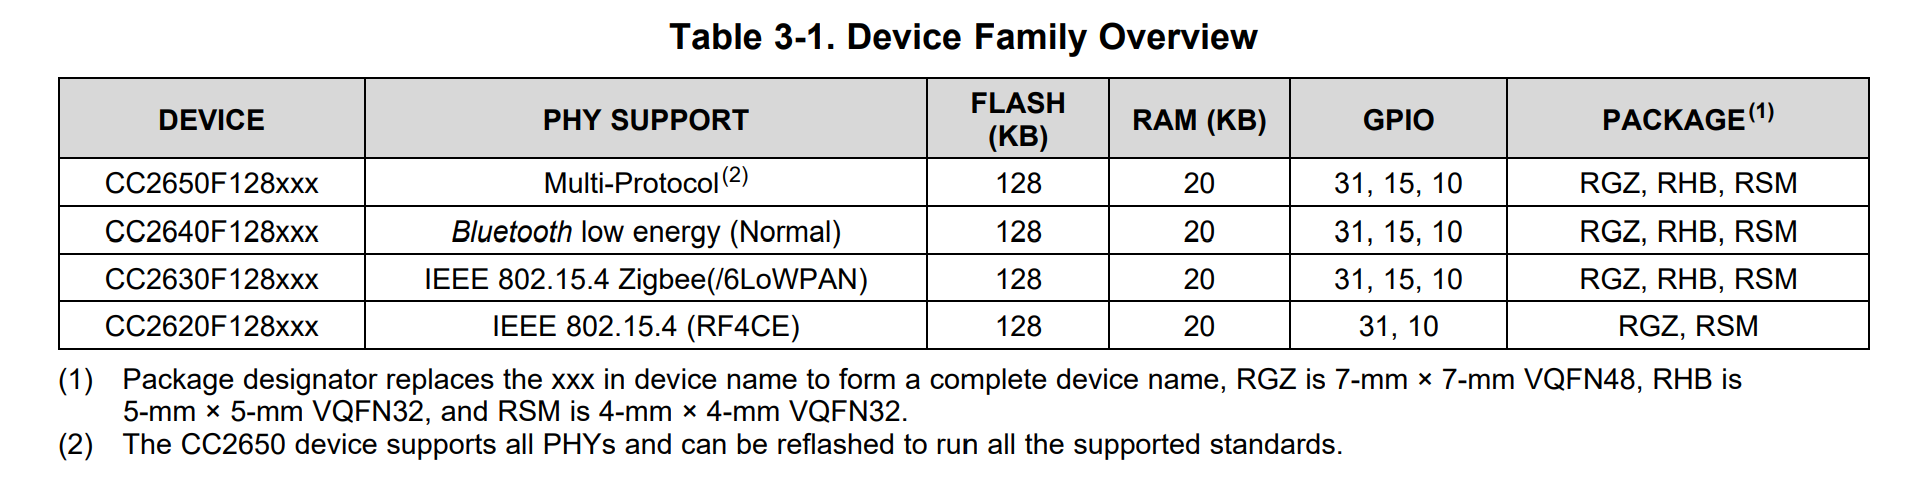
\includegraphics[width=1\textwidth]{media/table26xx.png}
  \caption{Test des Messagebrokers Mosquitto}
\end{figure}

Als Koordinator werden die Leistungsfähigeren Chips aus der 265X Reihe eingesetzt. ZigBee Geräte nutzen in manchen
Fällen Bluetooth LE zur Koppelung, daher ist die simultane Unterstüzung diesen Protokolls sinnvoll.

\begin{figure}[H]
  \centering
  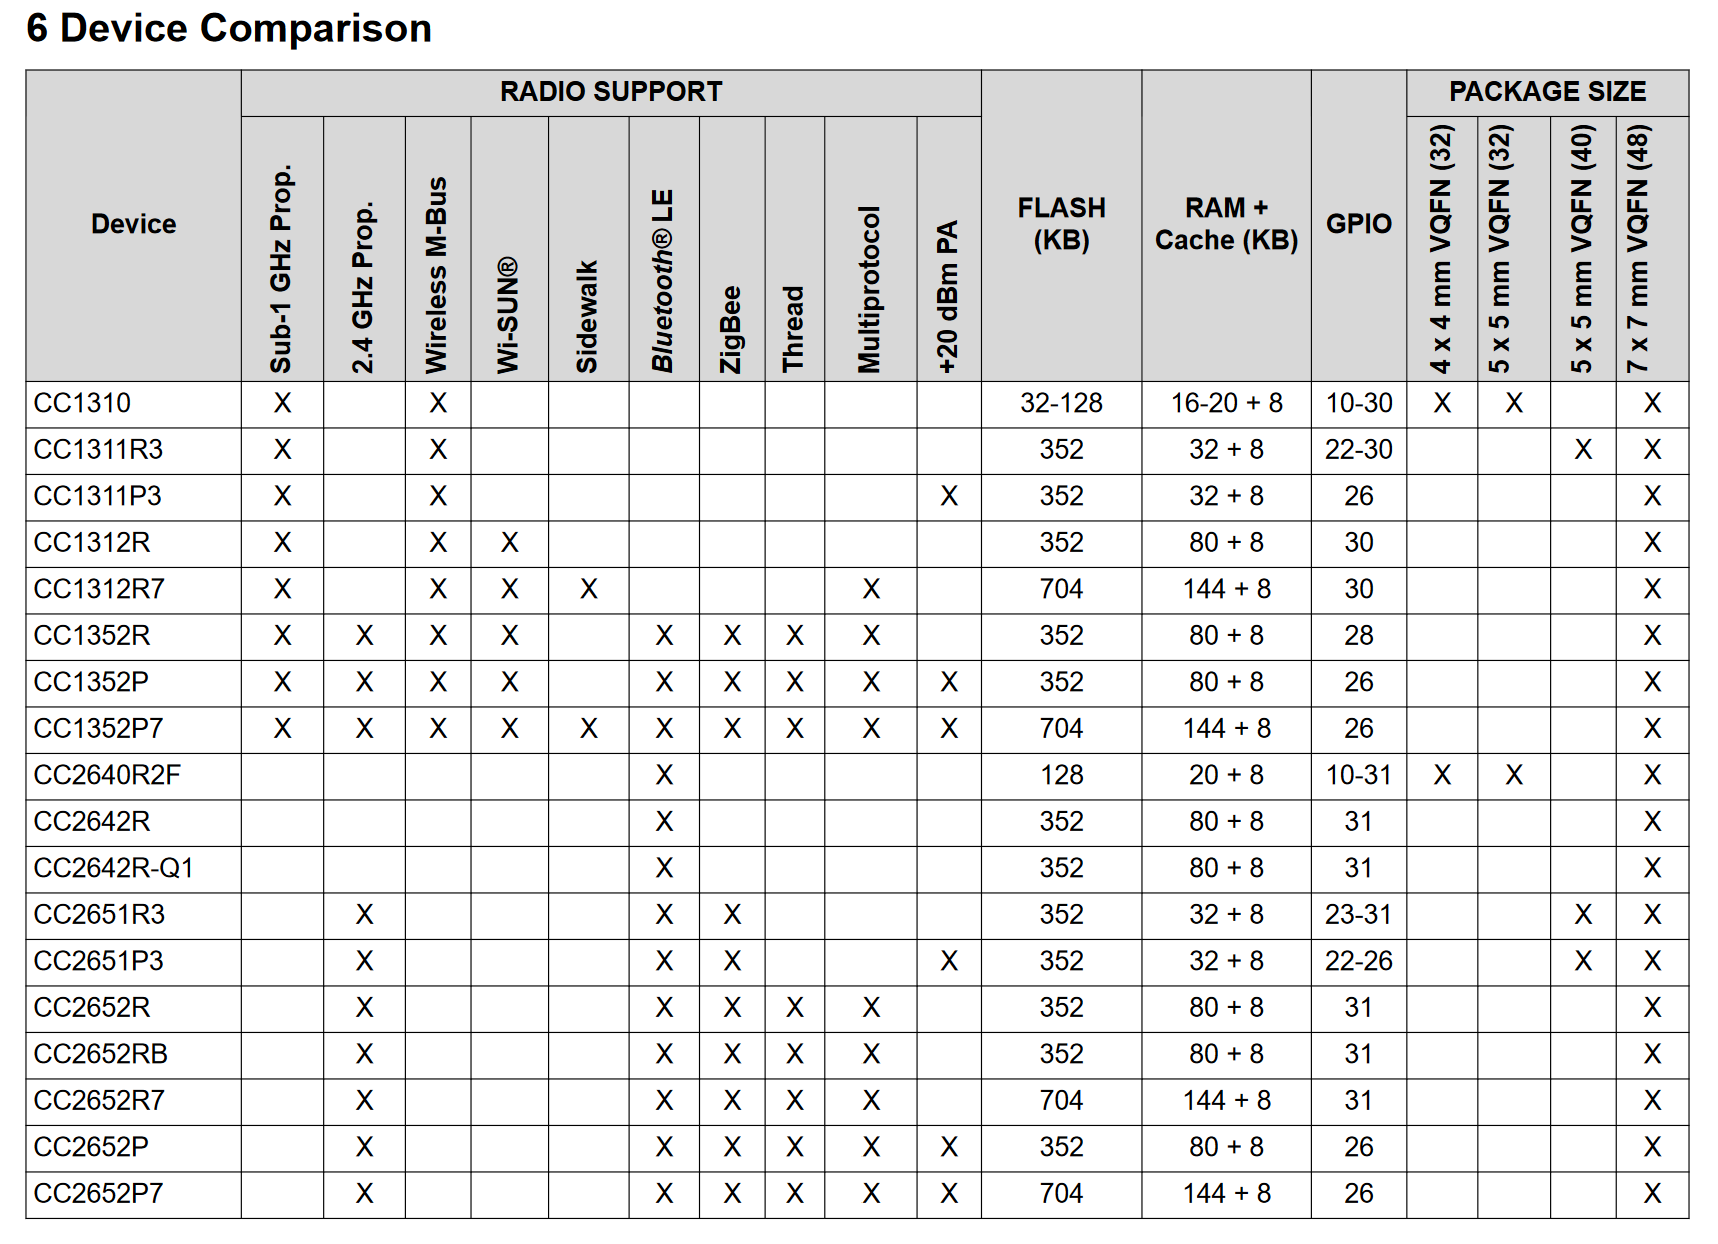
\includegraphics[width=1\textwidth]{media/table265x.png}
  \caption{Test des Messagebrokers Mosquitto}
\end{figure}

Hier in der Tabelle sind die unterstützten Protokolle der einzelnen Modelle sowie deren Leistungsfähigkeit aufgeführt.
Spannenderweise ist zu sehen, dass die Top Modelle schon den Standard Thread unterstützen, der vermutlich durch das
Projekt "Matter" erheblich an bedeutung gewinnt.

Texas Instruments bietet als Basis für ZigBee Eigententwicklungen eine Z-Stack Bibliothek. Diese stellt alle grundlegende 
Funktionen um das ZigBee Protokoll zu implementieren. Mit TexasInstruments Code Composer Studio steht eine IDE bereit,
um den Entwicklungsprozess zu unterstützen. Auf den entsprechend Leistungsfähigeren Chips lassen sich so noch zusätzliche
Funktionalitäten einprogrammieren.

Weiter Informationen: \url{https://www.ti.com/tool/Z-STACK#overview}

In dem OpenSource Projekt "zigbee2mqtt" werden ausschließlich Chips von Texas Instruments unterstützt. Es sei erwähnt, 
dass die meißten gängigen Anbieter von Microchips entsprechende Modelle im Angebot haben. 

\section{Versuchshardware}

\subsection{RaspberryPi}

Der RaspberryPi ist ein ARM basierter Computer im Mini-Format. Er dient in diesem Versuch als Server, der die Applikationen
hostet und gleichzeitig als Versuchs PC, von dem der Versuch aus ausgeführt wird. Die eingesetzten Dienste sind alle
als Webservice implementiert, und daher vollständig auf Kommandozeile parametrierbar, sowie mit WebGUI bedienbar.

Der RaspberryPi besitzt die Nutzer PC typtischen Schnittstellen wie Ethernet, HDMI, sowie USB. Als Hauptspeicher wird eine
SD-Karte eingestzt. Dies ist ein erheblicher Vorteil beim vorbereiten mehrerer RaspberryPis für den Versuch.

Auf dem RaspberryPi wird das Linux-basierte Betriebssystem RaspbyanOS eingesetzt. Durch die enorme Verbreitung ist
hier mit regelmäígen Updates in Zukunft zu rechnen.

\subsection{RaspberryPi Zigbee Hat}

Als Zigbee Koordinator kommt ein auf dem TI CC2652 basierendem RaspberryPi Hat vom Hersteller \grqq cod.m \grqq{} zum Einsatz. Dieser wurde vom Hersteller
zum Einsatz mit \grqq homegear \grqq{} oder \grqq zigbee2Mqtt \grqq{}. Ein Datenblatt sowie ein Manual ist im Anhang.

\subsection{CC2235 Sniffer Stick}

Mit diesem Stick wird die ZigBee Kommunikation zwischen dein einzelnen Devices sowie dem Koordinator mitgeschnitten auf einem bestimmten Kanal mitgeschnitten.
Es lässt sich beinahe jeder Texas Instruments ZigBee Chip bereits auf einen USB-Stick aufgelötet günstig aus China beziehen. 

\url{https://github.com/virtualabs/cc2531-killerbee-fw}

\subsection{Phillips Hue Komponenten}

Die Phillips Hue Serie setzt vollständig auf den ZigBee Standard auf. Die Produkte haben ein eigenes Öko-System mit entsprechender App und Gateway. Sie sind Kompatibel
zu dem Software-Gateway zigbee2mqtt.
Die Lampen werden in dem Versuch als Demonstrationsobjekte eingesetzt. Sie können Ein- und Ausgeschaltet werden, sowie gedimmt werden. Zusätzlich wird einer
Phillips Hie Fernbedienung verwendet, die zur Steuerung der Lampen dient.

\section{Eingesetzte Software}

\subsection{Raspbian OS}

RaspbianOS ist eine leichtgewichtige Linux Distribution, welche direkt vom Hersteller des RaspberryPis speziell auf die Bedürfnisse des Board angepasst werden. Es enthällt eine
Desktop Umgebung sowie die grundlegende Paketen. Es basiert auf Debian, damit sind auch die entsprechenden Paketquellen verfügbar.

\subsection{Docker}

Docker ist eine Container Umgebung, um Anwendungen containerisiert auf Linux-Servern laufen lassen zu können. Docker reduziert erheblich den Aufwand, 
Anwendungen auf Servern auszurollen. Alle Abhängigkeiten sind im Container enthalten, sodass hier keine Komplikationen mit anderen Anwendungen
zu befürchten sind. Prozesse laufen in eigenen Namespaces und sind dadurch abgekoppelt vom Host Betriebssystem. Im Unterschied zur Virtualisierung werden
Systemprozesse gemeinsam genutzt. Dadurch ist die Effizienz höher, als bei taditioneller Virtualisierung.

\subsection{zigbee2mqtt}

zigbee2mqtt ist ein offenes Softwareprojekt und stellt ein \grqq Software-Zigbee-Gateway \grqq dar. Es übernimmt die Funktionalität, die normalerweise entsprechende
\grqq Bridges \grqq übernehmen. Während traditionelle Bridges, wie zum Beispiel die Phillips Hue Bridge eine REST API zur Verfügung stellen um mit Ihren entsprechenden
Apps zu kommunizieren, macht zigbee2mqtt die Geräte per mqtt nach außen verfügbar. Auf abstrakterer Ebene bedeutet dies, das es ein Gateway zwischen einem Zigbee Netzwerk und
einem traditionellen IPv4 Netzwerk ist. Zur Steuerung und Visualisierung lassen sich per MQTT Anwendungen wie \grqq Homeassistant \grqq oder \grqq OpenHUB \grqq{} bzw. entsprechende
Eigenentwicklungen einsetzen.

Quellcode und Dokumentation: \url{https://github.com/Koenkk/zigbee2mqtt}
Homepage: \url{https://www.zigbee2mqtt.io/}

\subsubsection{TI CC Firmware}

Firmware für die Texas Instruments Chips, um diese als Koordinator einsetzen zu können. Die Firmware basiert auf dem Z-Stack von Texas Instruments. Sie wird fertig kompiliert
in einem Git-Repo angeboten. 

\subsubsection{zigbee-herdman}

Dieses Modul verbindet sich direkt mit dem Zigbee Adapter, und steuert Ihn über die \grqq TI zStack monitoring and test API \grqq{}. \cite{zstack}

Zur verdeutlichung, wie dies in Realität aussieht, hier ein Ausschnitt aus der API Dokumentation.

\begin{figure}[H]
  \centering
  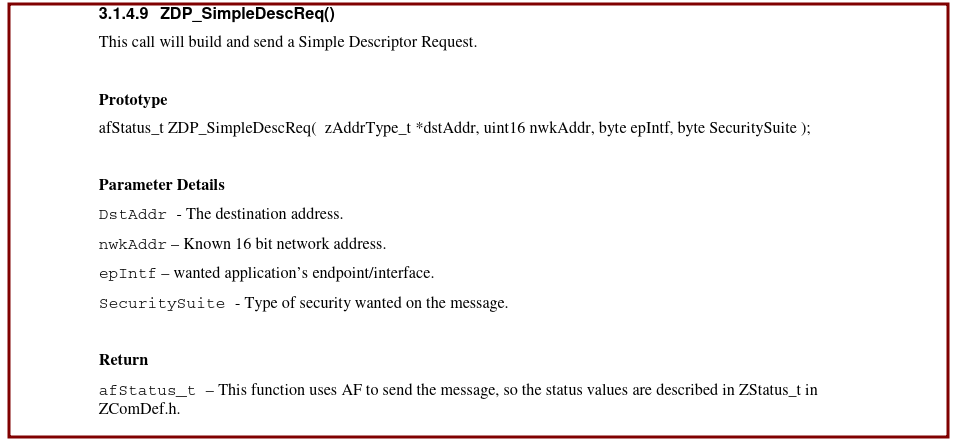
\includegraphics[width=1\textwidth]{media/z-stack-api-excerpt.png}
  \caption{Z-Stack API Auszug}
\end{figure}

In diesem Beispiel wird beschrieben, wie man einen SimpleDescriptor-Request an ein Zigbee-Device versendet. Dieser Aufruf ist entsprechend Parametrierbar,
und wird zur Abfrage der verfügbaren Endpunkte eines Gerätes nach dessen Beitritt in das Netzwerk abgefragt.

\subsubsection{zigbee-herdman-converters}

Dieser Konverter kann proprietäre Cluster die durch Geräte exposed werden umwandeln in Standard Cluster. Mit diesem Converter lassen sich proprietäre Cluster von Geräte
so adaptieren, dass sie nach Wunsch gesteuert und ausgelesen werden können.

\subsubsection{zigbee2mqtt}

Das Hauptmodul stellt die WebGui sowie eine Webanwendung mit einer SQLite Datenbank. Die Webanwendung und die Datenbank
verwalten den Zustand des Netzwerkes und die angebundenen Geräte. Die WebGUI dient zur Administration des Koordinators. 

\begin{figure}[H]
  \centering
  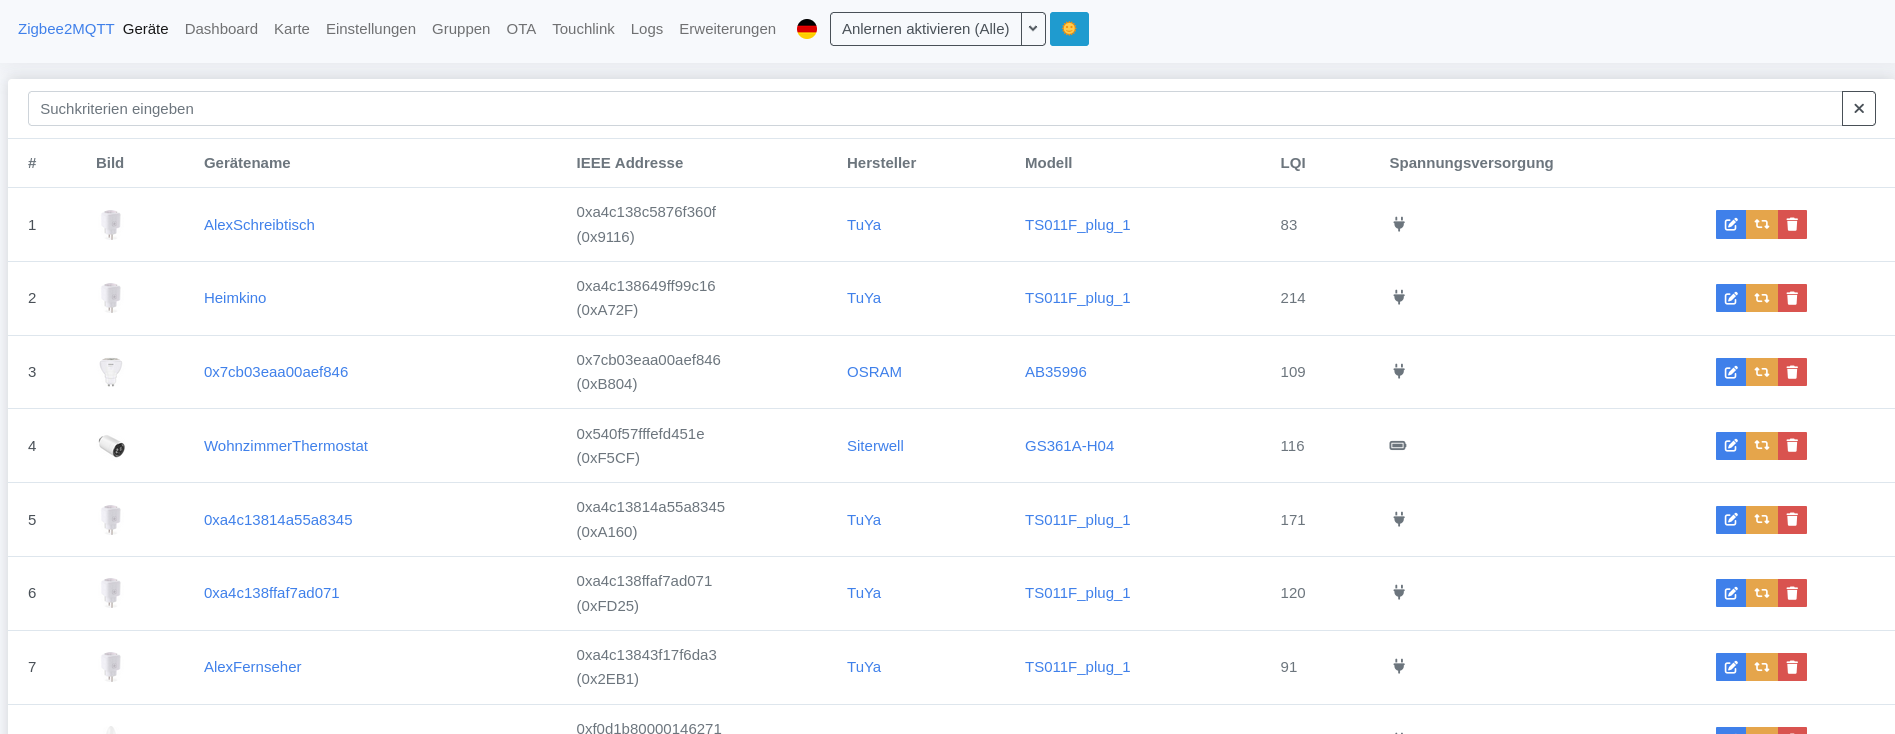
\includegraphics[width=1\textwidth]{media/z2m.png}
  \caption{zigbee2mqtt Webfrontend}
\end{figure}

Die WebGUI enthällt eine große Anzahl von Funktionen, die weitaus tiefer reichen als für die Nutzung notwendig sind.
Prinzipiell sind die meißten ZigBee Geräte Kompatibel, wenn ein Community Mitglied dieses bereits in der Anwendung
angelegt hat. Es ist auch möglich, eigene Beschreibungen für nich nicht unterstützte Geräte zu erstellen.\\

\begin{figure}[H]
  \centering
  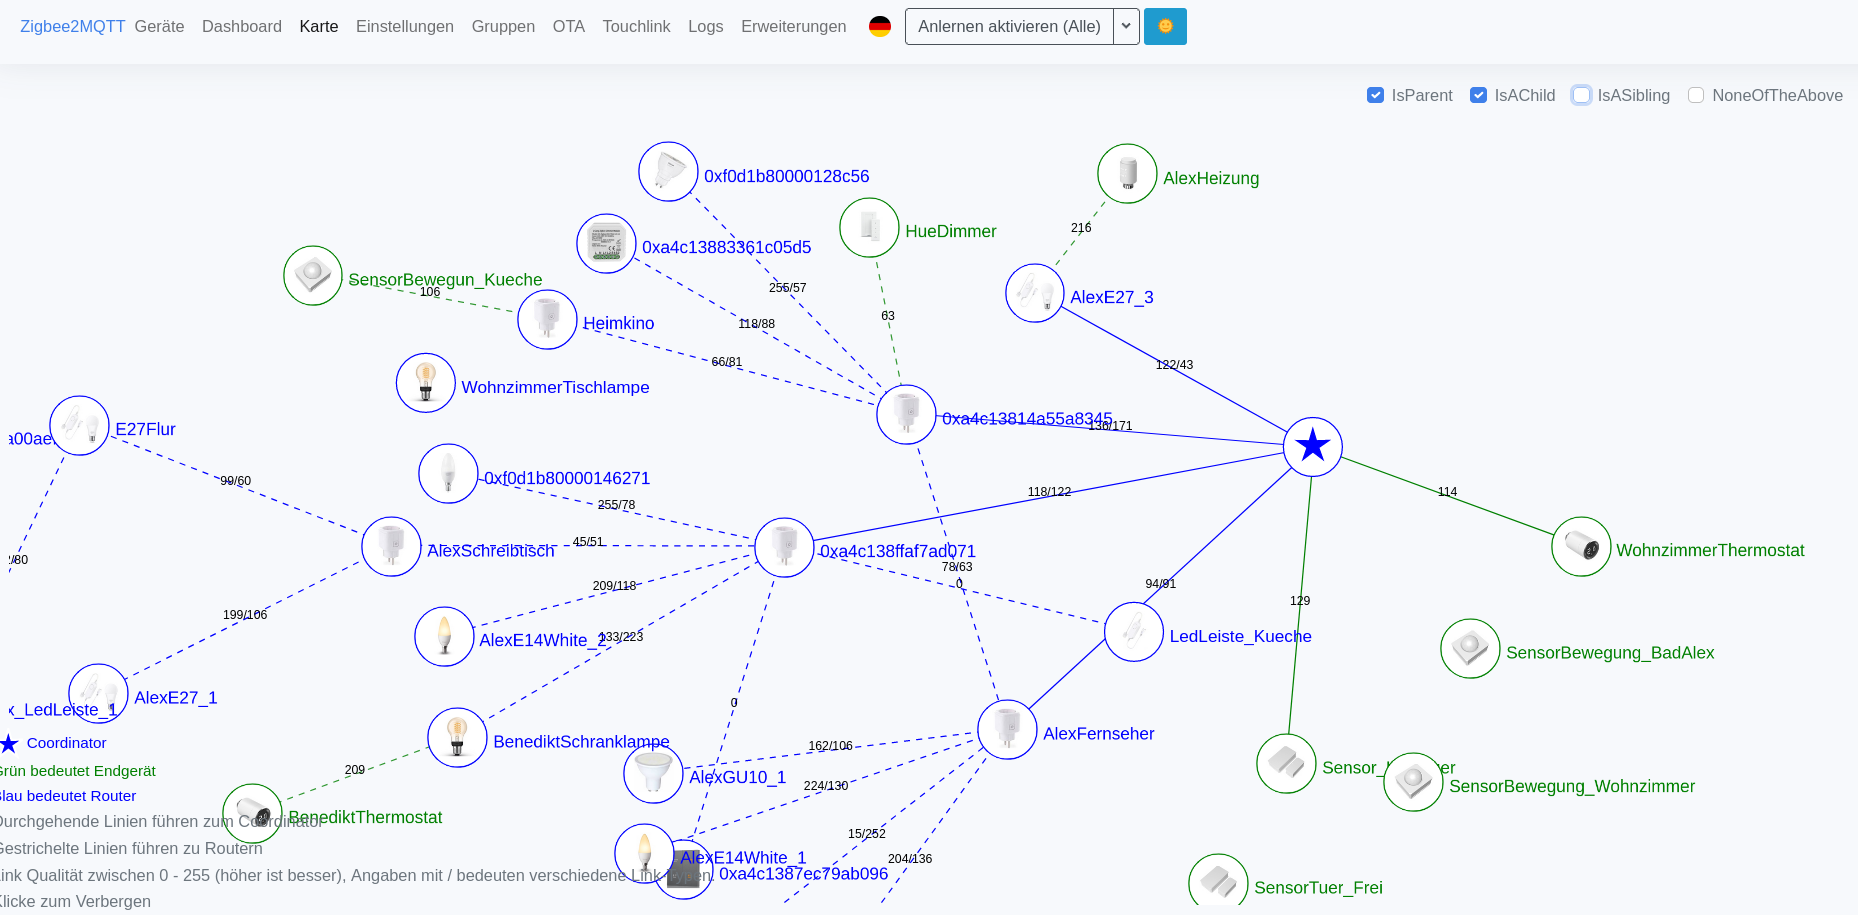
\includegraphics[width=1\textwidth]{media/z2m-map.png}
  \caption{zigbee2mqtt Netzwerkvisualisierung}
\end{figure}

Das Netzwerk lässt sich in einer dynamischen Übersicht visualisieren. Hier die aktiven Verbindung zwischen den Geräten. 

\subsection{Wireshark}

Wireshark ist eine quelloffene Anwendung um Datenstöme Mitzuschneiden und zu Untersuchen. Es kann durch Verwendung
von Packetsniffern wie nPcap verschiedenste Medien wie zum Beispiel Ethernet und USB mit entsprechenden Protokollen
verarbeiten.

\subsection{zbWireshark}

Dies ist eine Script aus einer Git-Hub Scriptsammlung. Mit diesem Script lässt sich Wireshark starten und anschließend Pakete über den 
 ZigBee Sniffer Stick mitschreiben.

\url{https://github.com/silicrax/killerbee/tree/master/tools}

\subsection{Ansible}
